\chapter{Regression}
    % Authors: Jiachen Zhu, Rafael Moraes, Kabir Singh; 2019-02-19
    
    
    
    
    
        
    The following code shows some experiments on how to use neural networks for regression.
    \section{Create the data}
    \begin{minted}{python}
import random
import torch
from torch import nn, optim
import math
from IPython import display
from plot_lib import plot_data, plot_model, set_default
from matplotlib import pyplot as plt

set_default()        
        \end{minted}
        
        \begin{minted}{python}
seed = 12345
random.seed(seed)
torch.manual_seed(seed)
N = 1000  # num_samples_per_class
D = 1  # dimensions
C = 1  # num_classes
H = 100  # num_hidden_units
X = torch.unsqueeze(torch.linspace(-1, 1, 100), dim=1)
y = X.pow(3) + 0.3 * torch.rand(X.size())
        \end{minted}
        
        \begin{minted}{python}
print("Shapes:")
print("X:", tuple(X.size()))
print("y:", tuple(y.size()))
        \end{minted}
        
        \begin{minted}{python}
plt.scatter(X.numpy(), y.numpy())
plt.axis('equal')        
        \end{minted}
        Since we want to do a Regression, we treat the data as one-dimensional (D = 1) and the output as one-dimensional (C = 1).
        
        % Linear Model
        \section{Linear Model}
        \begin{minted}{python}
learning_rate = 1e-3
lambda_l2 = 1e-5

device = torch.device("cuda:0" if torch.cuda.is_available() else "cpu")
# nn package to create our linear model
# each Linear module has a weight and bias
model = nn.Sequential(
    nn.Linear(D, H),
    nn.Linear(H, C)
)
model.to(device) # Convert to CUDA
# nn package also has different loss functions.
# we use MSE loss for our regression task
criterion = torch.nn.MSELoss()
# we use the optim package to apply
# stochastic gradient descent for our parameter updates
optimizer = torch.optim.SGD(model.parameters(), lr=learning_rate, weight_decay=lambda_l2) # built-in L2
        \end{minted}
        
        \begin{minted}{python}
for t in range(1000):    
    # Feed forward to get the logits
    y_pred = model(X)    
    # Compute the loss (MSE)
    loss = criterion(y_pred, y)
    print("[EPOCH]: %i, [LOSS or MSE]: %.6f" % (t, loss.item()))
    display.clear_output(wait=True)    
    # zero the gradients before running
    # the backward pass.
    optimizer.zero_grad()
    # Backward pass to compute the gradient
    # of loss w.r.t our learnable params. 
    loss.backward()    
    # Update params
    optimizer.step()
        \end{minted}
        \begin{minted}{python}
plt.scatter(X.data.numpy(), y.data.numpy())
plt.plot(X.data.numpy(), y_pred.data.numpy(), 'r-', lw=5)
plt.axis('equal');        
        \end{minted}
        When using the simple linear model, there are two \texttt{nn.Linear} layers without any non-linearity, so this is equivalent to a single linear layer and the output is a straight line. This is called Linear Regression.
    
        \begin{figure}[H]
        \begin{center}
        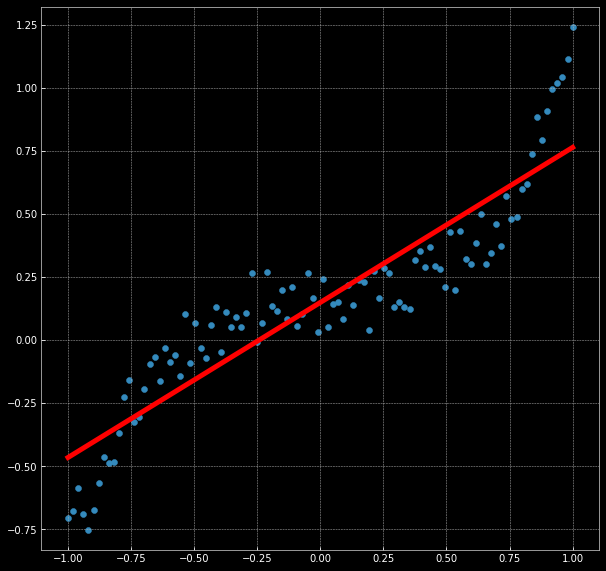
\includegraphics[width=200pt]{labs/03/images/05-first_reg.png}
        \end{center} 
        \caption{Regression using linear NN model (without non-linearity).}
        % \label{fig:mon}
        \end{figure}
        
        % Two-layered network
        \section{Two-layered network}
        \begin{minted}{python}
learning_rate = 1e-3
lambda_l2 = 1e-5
# Number of networks
n_networks = 5
models = list()
y_pretrain = list()
# nn package also has different loss functions.
# we use MSE for a regression task
criterion = torch.nn.MSELoss()

for mod in range(n_networks):
    # nn package to create our linear model
    # each Linear module has a weight and bias
    model = nn.Sequential(
        nn.Linear(D, H),
        nn.ReLU(),
        nn.Linear(H, C)
    )
    model.to(device)
    # Append models
    models.append(model)
    # we use the optim package to apply
    # ADAM for our parameter updates
    optimizer = torch.optim.Adam(model.parameters(), lr=learning_rate, weight_decay=lambda_l2) # built-in L2
    # e = 1.  # plotting purpose
    # Training
    for t in range(1000):
        # Feed forward to get the logits
        y_pred = model(X)     
        # Append pre-train output
        if t == 0:
            y_pretrain.append(y_pred)
        # Compute the loss and accuracy
        loss = criterion(y_pred, y)
        print(f"[MODEL]: {mod + 1}, [EPOCH]: {t}, [LOSS]: {loss.item():.6f}")
        display.clear_output(wait=True)
        # zero the gradients before running
        # the backward pass.
        optimizer.zero_grad()
        # Backward pass to compute the gradient
        # of loss w.r.t our learnable params. 
        loss.backward()
        # Update params
        optimizer.step()        
        \end{minted}
        
        % Before training
        \section{Predictions: Before Training}
         \begin{minted}{python}
for y_pretrain_idx in y_pretrain:
    # New X that ranges from -5 to 5 instead of -1 to 1
    X_new = torch.unsqueeze(torch.linspace(-2, 2, 100), dim=1)
        
    plt.plot(X_new.data.numpy(), y_pretrain_idx.data.numpy(), 'r-', lw=1)

plt.scatter(X.data.numpy(), y.data.numpy())
plt.axis('equal')
        \end{minted}

        \begin{figure}[H]
        \begin{center}
        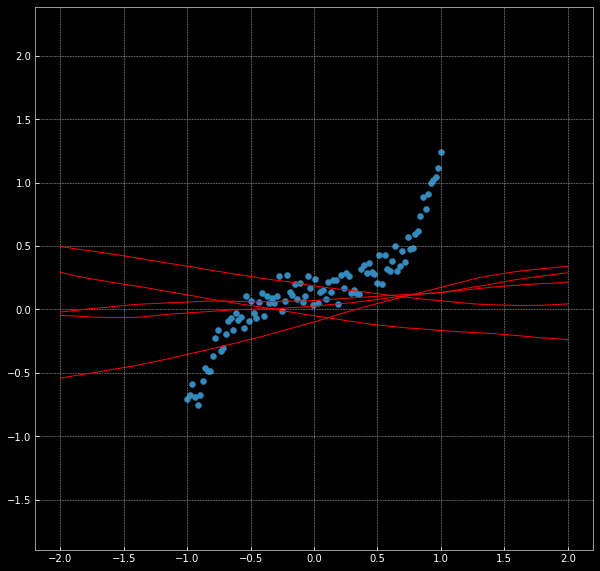
\includegraphics[width=200pt]{labs/03/images/05-random_at_first.png}
        \end{center} 
        \caption{Random weights at first.}
        % \label{fig:mon}
        \end{figure}

        % After training
        \section{Predictions: After Training}
        \begin{minted}{python}
for model in models:
    # New X that ranges from -5 to 5 instead of -1 to 1
    X_new = torch.unsqueeze(torch.linspace(-1, 1, 100), dim=1)

    # Getting predictions from input
    with torch.no_grad():
        y_pred = model(X_new)
        
    plt.plot(X_new.data.numpy(), y_pred.data.numpy(), 'r-', lw=1)
plt.scatter(X.data.numpy(), y.data.numpy())
        \end{minted}
        When we add a ReLU between the two \texttt{nn.Linear} layers, the model now is equivalent to having segments of different straight lines, "selected" by the ReLU activation. 
        Now we can model more complex functions by using these segments; the more hidden units (i.e. ReLU units), the more complex (i.e. more edges) the final function will be. This is called Piecewise-linear Regression.
        \begin{figure}[H]
        \begin{center}
        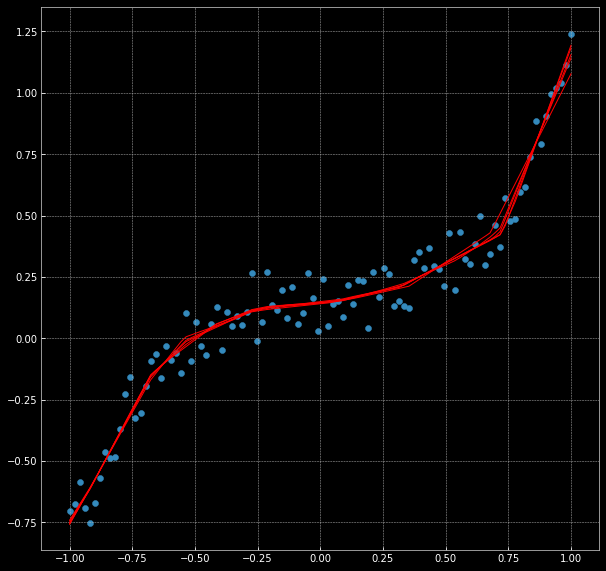
\includegraphics[width=200pt]{labs/03/images/05-piecewise_reg.png}
        \end{center} 
        \caption{Regression using piecewise-linear model (with ReLU non-linearity).}
        % \label{fig:mon}
        \end{figure}
        Out of the interval of the train data the variance explodes. 
        We have no information as to what should happen there, so the model does not introduce any new edge and the slopes of the last segments (to the left and right of the data) is extended.
        
% ############################# 
\chapter{Convolutional Networks}
    % Authors: Jiachen Zhu, Rafael Moraes, Kabir Singh; 2019-02-19
    
    In this chapter, two models are presented:
    \begin{itemize}
        \item A fully-connected network 
        \item A convolutional network with the same number of parameters as the fully-connected network.
    \end{itemize}
    Through two experiments, we show that:
    \begin{itemize}
        \item The ConvNet makes better use of its parameters by exploiting the properties of natural data, thus achieving a higher accuracy than the fully-connected network.
        \item After random shuffling the pixels of the images in the same way for all inputs, the fully-connected network achieves a similar performance, while the CNN performed worse than the FC network due to the input losing the natural data properties that made convolutions work well.
    \end{itemize}

    \section{Libraries}
    To run the code in this chapter, we need import all necessary libraries at first.
    Apart from \emph{PyTorch}, we also need the \emph{torchvision} library.
    It consists of some popular datasets for computer vision, and also includes some common image transformation functions.
    \begin{minted}{python}
import torch
import torch.nn as nn
import torch.nn.functional as F
import torch.optim as optim
import torchvision
    \end{minted}

    \section{Dataset}
    % Authors: Jiachen Zhu, Rafael Moraes, Kabir Singh; 2019-02-19
    In the chapter, we will use the MNIST handwritten digit database to test our models.
    The dataset could be imported easily from the \emph{torchvision} library.
    \begin{minted}{python}
input_size  = 28 * 28   # images are 28x28 pixels
output_size = 10      # there are 10 classes

# The output of torchvision datasets are PILImage images of range [0, 1].
# We transform them to Tensors of normalized range [-1, 1].
transform = torchvision.transforms.Compose([
    torchvision.transforms.ToTensor(),
    torchvision.transforms.Normalize((0.1307,), (0.3081,))])
train_set = torchvision.datasets.MNIST(root='./data', train=True, download=True, 
    transform=transform)
test_set = torchvision.datasets.MNIST(root='./data', train=False, download=True,
    transform=transform)
    \end{minted}
    After getting the MNIST dataset from \emph{torchvision}, we need to create data loaders for training set and test set.
    \begin{minted}{python} 
train_loader = torch.utils.data.DataLoader(train_set, batch_size=64, shuffle=True)
test_loader = torch.utils.data.DataLoader(test_set, batch_size=64, shuffle=False)
    \end{minted}
    
    \section{CNN vs Fully-Connected Networks}
    % Authors: Jiachen Zhu, Rafael Moraes, Kabir Singh; 2019-02-19
        We create two image classification models, one only use the linear layers and the other use convolutional layers.
        \begin{minted}{python}
class FC2Layer(nn.Module):
    def __init__(self, input_size, n_hidden, output_size):
        super(FC2Layer, self).__init__()
        self.input_size = input_size
        self.network = nn.Sequential(
            nn.Linear(input_size, n_hidden), 
            nn.ReLU(), 
            nn.Linear(n_hidden, n_hidden), 
            nn.ReLU(), 
            nn.Linear(n_hidden, output_size), 
            nn.LogSoftmax(dim=1)
        )

    def forward(self, x):
        x = x.view(-1, self.input_size)
        return self.network(x)
    
class CNN(nn.Module):
    def __init__(self, input_size, n_feature, output_size):
        super(CNN, self).__init__()
        self.n_feature = n_feature
        self.conv1 = nn.Conv2d(in_channels=1, out_channels=n_feature, kernel_size=5)
        self.conv2 = nn.Conv2d(n_feature, n_feature, kernel_size=5)
        self.fc1 = nn.Linear(n_feature*4*4, 50)
        self.fc2 = nn.Linear(50, 10)
        
    def forward(self, x, verbose=False):
        x = self.conv1(x)
        x = F.relu(x)
        x = F.max_pool2d(x, kernel_size=2)
        x = self.conv2(x)
        x = F.relu(x)
        x = F.max_pool2d(x, kernel_size=2)
        x = x.view(-1, self.n_feature*4*4)
        x = self.fc1(x)
        x = F.relu(x)
        x = self.fc2(x)
        x = F.log_softmax(x, dim=1)
        return x
        \end{minted}
        Then, we can define the corresponding train and test functions for both models.
        The \texttt{perm} parameter will be used to permute pixels in the second experiment.
        \begin{minted}{python}
def train(epoch, model, perm=torch.arange(0, 784).long()):
    model.train()
    for batch_idx, (data, target) in enumerate(train_loader):
        # permute pixels
        data = data.view(-1, 28*28)
        data = data[:, perm]
        data = data.view(-1, 1, 28, 28)

        optimizer.zero_grad()
        output = model(data)
        loss = F.nll_loss(output, target)
        loss.backward()
        optimizer.step()
        if batch_idx % 100 == 0:
            print('Train Epoch: {} [{}/{} ({:.0f})] tLoss: {:.6f}'.format(
                epoch, batch_idx * len(data), len(train_loader.dataset),
                100. * batch_idx / len(train_loader), loss.item()))
            
def test(model, perm=torch.arange(0, 784).long()):
    model.eval()
    test_loss = 0
    correct = 0
    for data, target in test_loader:
        # permute pixels
        data = data.view(-1, 28*28)
        data = data[:, perm]
        data = data.view(-1, 1, 28, 28)
        
        output = model(data)
        test_loss += F.nll_loss(output, target, reduction='sum').item() # sum up batch loss                                               
        pred = output.data.max(1, keepdim=True)[1] # get the index of the max log-probability           
        correct += pred.eq(target.data.view_as(pred)).cpu().sum().item()

    test_loss /= len(test_loader.dataset)
    accuracy = 100. * correct / len(test_loader.dataset)
    print('Test set: Average loss: {:.4f}, Accuracy: {}/{} ({:.0f}%)'.format(
        test_loss, correct, len(test_loader.dataset),
        accuracy))
        \end{minted}
        
        \subsection{Experiment 1: Regular Images}
        % Authors: Jiachen Zhu, Rafael Moraes, Kabir Singh; 2019-02-19
        In the first experiment, we will train both models with regular images.
        The CNN model:
        \begin{minted}{python}
# Training settings 
n_features = 6 # number of feature maps

model_cnn = CNN(input_size, n_features, output_size)
optimizer = optim.SGD(model_cnn.parameters(), lr=0.01, momentum=0.5)

for epoch in range(0, 1):
    train(epoch, model_cnn)
    test(model_cnn)
        \end{minted}
        The result:
        \begin{verbatim}
Train Epoch: 0 [0/60000 (0)] tLoss: 2.320940
Train Epoch: 0 [6400/60000 (11)] tLoss: 2.251726
Train Epoch: 0 [12800/60000 (21)] tLoss: 0.926804
Train Epoch: 0 [19200/60000 (32)] tLoss: 0.602818
Train Epoch: 0 [25600/60000 (43)] tLoss: 0.638813
Train Epoch: 0 [32000/60000 (53)] tLoss: 0.562240
Train Epoch: 0 [38400/60000 (64)] tLoss: 0.189035
Train Epoch: 0 [44800/60000 (75)] tLoss: 0.381978
Train Epoch: 0 [51200/60000 (85)] tLoss: 0.202108
Train Epoch: 0 [57600/60000 (96)] tLoss: 0.393331
Test set: Average loss: 0.2206, Accuracy: 9347/10000 (93%)
        \end{verbatim}
        The fully-connected network:
        \begin{minted}{python}
n_hidden = 8 # number of hidden units

model_fnn = FC2Layer(input_size, n_hidden, output_size)
optimizer = optim.SGD(model_fnn.parameters(), lr=0.01, momentum=0.5)

for epoch in range(0, 1):
    train(epoch, model_fnn)
    test(model_fnn)
        \end{minted}
        The result:
        \begin{verbatim}
Train Epoch: 0 [0/60000 (0)] tLoss: 2.352721
Train Epoch: 0 [6400/60000 (11)] tLoss: 1.887923
Train Epoch: 0 [12800/60000 (21)] tLoss: 1.216436
Train Epoch: 0 [19200/60000 (32)] tLoss: 0.964433
Train Epoch: 0 [25600/60000 (43)] tLoss: 0.776250
Train Epoch: 0 [32000/60000 (53)] tLoss: 0.598156
Train Epoch: 0 [38400/60000 (64)] tLoss: 0.527515
Train Epoch: 0 [44800/60000 (75)] tLoss: 0.407989
Train Epoch: 0 [51200/60000 (85)] tLoss: 0.417804
Train Epoch: 0 [57600/60000 (96)] tLoss: 0.485479
Test set: Average loss: 0.4804, Accuracy: 8625/10000 (86%)
        \end{verbatim}
        From Experiment 1, we could see that CNN is better than fully-connected network on regular image classification.

        \subsection{Experiment 2: Permuted Pixels}
        % Authors: Jiachen Zhu, Rafael Moraes, Kabir Singh; 2019-02-19
        In the second experiment, we permute the pixels in a regular image, thereby losing locality in the image data.
        In this setup, the CNN should perform worse than itself with regular images, and the performance of fully-connected network should not have too much of difference.
        
        \begin{minted}{python}
perm = torch.randperm(784)
for i in range(10):
    image, _ = train_loader.dataset.__getitem__(i)
    # permute pixels
    image_perm = image.view(-1, 28*28).clone()
    image_perm = image_perm[:, perm]
    image_perm = image_perm.view(-1, 1, 28, 28)

# Training settings 
n_features = 6 # number of feature maps

model_cnn = CNN(input_size, n_features, output_size)
optimizer = optim.SGD(model_cnn.parameters(), lr=0.01, momentum=0.5)

for epoch in range(0, 1):
    train(epoch, model_cnn, perm)
    test(model_cnn, perm)

n_hidden = 8    # number of hidden units

model_fnn = FC2Layer(input_size, n_hidden, output_size)
optimizer = optim.SGD(model_fnn.parameters(), lr=0.01, momentum=0.5)

for epoch in range(0, 1):
    train(epoch, model_fnn, perm)
    test(model_fnn, perm)
        \end{minted}
        The training result for CNN:
        \begin{verbatim}
Train Epoch: 0 [0/60000 (0)] tLoss: 2.311677
Train Epoch: 0 [6400/60000 (11)] tLoss: 2.282326
Train Epoch: 0 [12800/60000 (21)] tLoss: 2.209269
Train Epoch: 0 [19200/60000 (32)] tLoss: 2.039113
Train Epoch: 0 [25600/60000 (43)] tLoss: 1.641617
Train Epoch: 0 [32000/60000 (53)] tLoss: 1.230703
Train Epoch: 0 [38400/60000 (64)] tLoss: 0.967219
Train Epoch: 0 [44800/60000 (75)] tLoss: 0.741154
Train Epoch: 0 [51200/60000 (85)] tLoss: 0.711306
Train Epoch: 0 [57600/60000 (96)] tLoss: 0.436662
Test set: Average loss: 0.5632, Accuracy: 8229/10000 (82%)
        \end{verbatim}
        The training result for fully-connected network:
        \begin{verbatim}
Train Epoch: 0 [0/60000 (0)] tLoss: 2.280286
Train Epoch: 0 [6400/60000 (11)] tLoss: 1.973936
Train Epoch: 0 [12800/60000 (21)] tLoss: 1.469295
Train Epoch: 0 [19200/60000 (32)] tLoss: 1.052585
Train Epoch: 0 [25600/60000 (43)] tLoss: 0.991563
Train Epoch: 0 [32000/60000 (53)] tLoss: 0.638042
Train Epoch: 0 [38400/60000 (64)] tLoss: 0.472083
Train Epoch: 0 [44800/60000 (75)] tLoss: 0.382082
Train Epoch: 0 [51200/60000 (85)] tLoss: 0.436203
Train Epoch: 0 [57600/60000 (96)] tLoss: 0.561125
Test set: Average loss: 0.4971, Accuracy: 8559/10000 (86%)
        \end{verbatim}
        The results show that convolutional network makes the assumption that pixels lie on a grid are stationary or local.
        It loses performance when this assumption is wrong.
        The fully-connected network does not make this assumption.
        It does less well, or approximately the same, when the assumption is true, since it doesn't take advantage of this prior knowledge. 